\section{Hardware choices and limitations}\label{sec:hardware}

This section describes the choices made for the project in terms of which hardware is required to construct the \projname{} prototype. In order for the robot to solve the tasks described in \secref{sec:system_definition}, some specific hardware is required. The hardware required for the robot is:

\begin{itemize}
\item Two motors to drive and steer the robot.
\item Two motors for collecting objects.
\item Two sensors to ensure that the robot stays inside the boundaries of the environment.
\item One sensor to detect objects.
\item One sensor for movement precision.
\end{itemize}

There exist a number of available sensors and actuators for the LEGO NXT. These sensors gives the NXT robots the ability to perform various actions. For the required tasks, it has been chosen to use the interactive servo motors for driving, steering, and the collection of objects. The colour sensor is well suited to ensure that the robot can detect the environment boundaries. For detecting objects, the ultrasonic sensor has been chosen, as the robot is required to know when an object is present and should be collected, as well as the distance to the detected object. Finally, to help ensure precise movement, the HiTechnic NXT Compass sensor is used.

Because the NXT brick only has output sockets for three motors, and the \projname{} will use at least four, two NXT bricks are required. This will require communication between the bricks, which is possible due to the NXT Brick's integrated Bluetooth, which allows interaction between the multiple NXT Bricks in a master-slave relationship with a maximum of 3 slaves pr. master. This allows the master-brick to send commands to the slave-bricks' output sockets and because of that, a single brick is able control more than the three motors a single NXT Brick otherwise would be limited to~\citep{lego_edu_guide}.

\subsection{Hardware test} \label{sec:hardware_test}
In order to know the capabilities and limitations of the hardware, some tests were conducted. Testing environments were set up to test the individual hardware devices. The early tests were created in LabView and transferred to the NXT brick. These used the original LEGO NXT firmware. During the test the LEGO Brick would write all the results into a file, which later would be transferred into LabView for analysis. 

Further tests were conducted using the data logging feature. A Bluetooth connection is established between the NXT brick and a PC, and while the robot is running, the outputs from the sensors and motors are logged and sent to the PC. The data can be saved in a .csv file and converted into graphs, which makes for easy analysis.

\subsubsection{Ultrasonic sensor} \label{sec:ultrasonic_sensor}
The ultrasonic sensor emits an ultrasonic sound wave and measures the time it takes for the wave to impact on an object and return to the sensor. Depending on the time taken, the sensor can measure the distance from the sensor to the detected object~\citep{lego_education}. 

\begin{figure}[H]
     \center{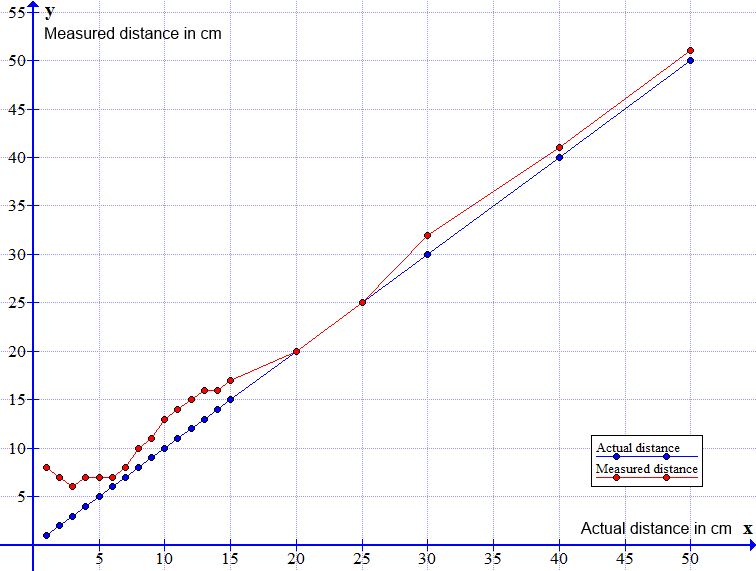
\includegraphics[width=320pt]
     {graphics/DistanceGraph.png}}
     \caption{\label{fig:ultrasonic_sensor_test_graph} The actual distance and the measured distance from the ultrasonic sensor test.}
\end{figure}

The ultrasonic sensor was tested at different distances to measure the accuracy. The test was performed stationary and every 25 ms it sends out a pulse, for 250 seconds, resulting in 1000 pulses, which would give a significant average of the distance. \appref{app:ultrasonic_sensor_test} shows the raw values observed during the test, which has been converted into the graph seen in \figref{fig:ultrasonic_sensor_test_graph}. The graph shows values from the tests from 1 cm to 50 cm. This test was performed using LabView.

\begin{figure}[H]
     \center{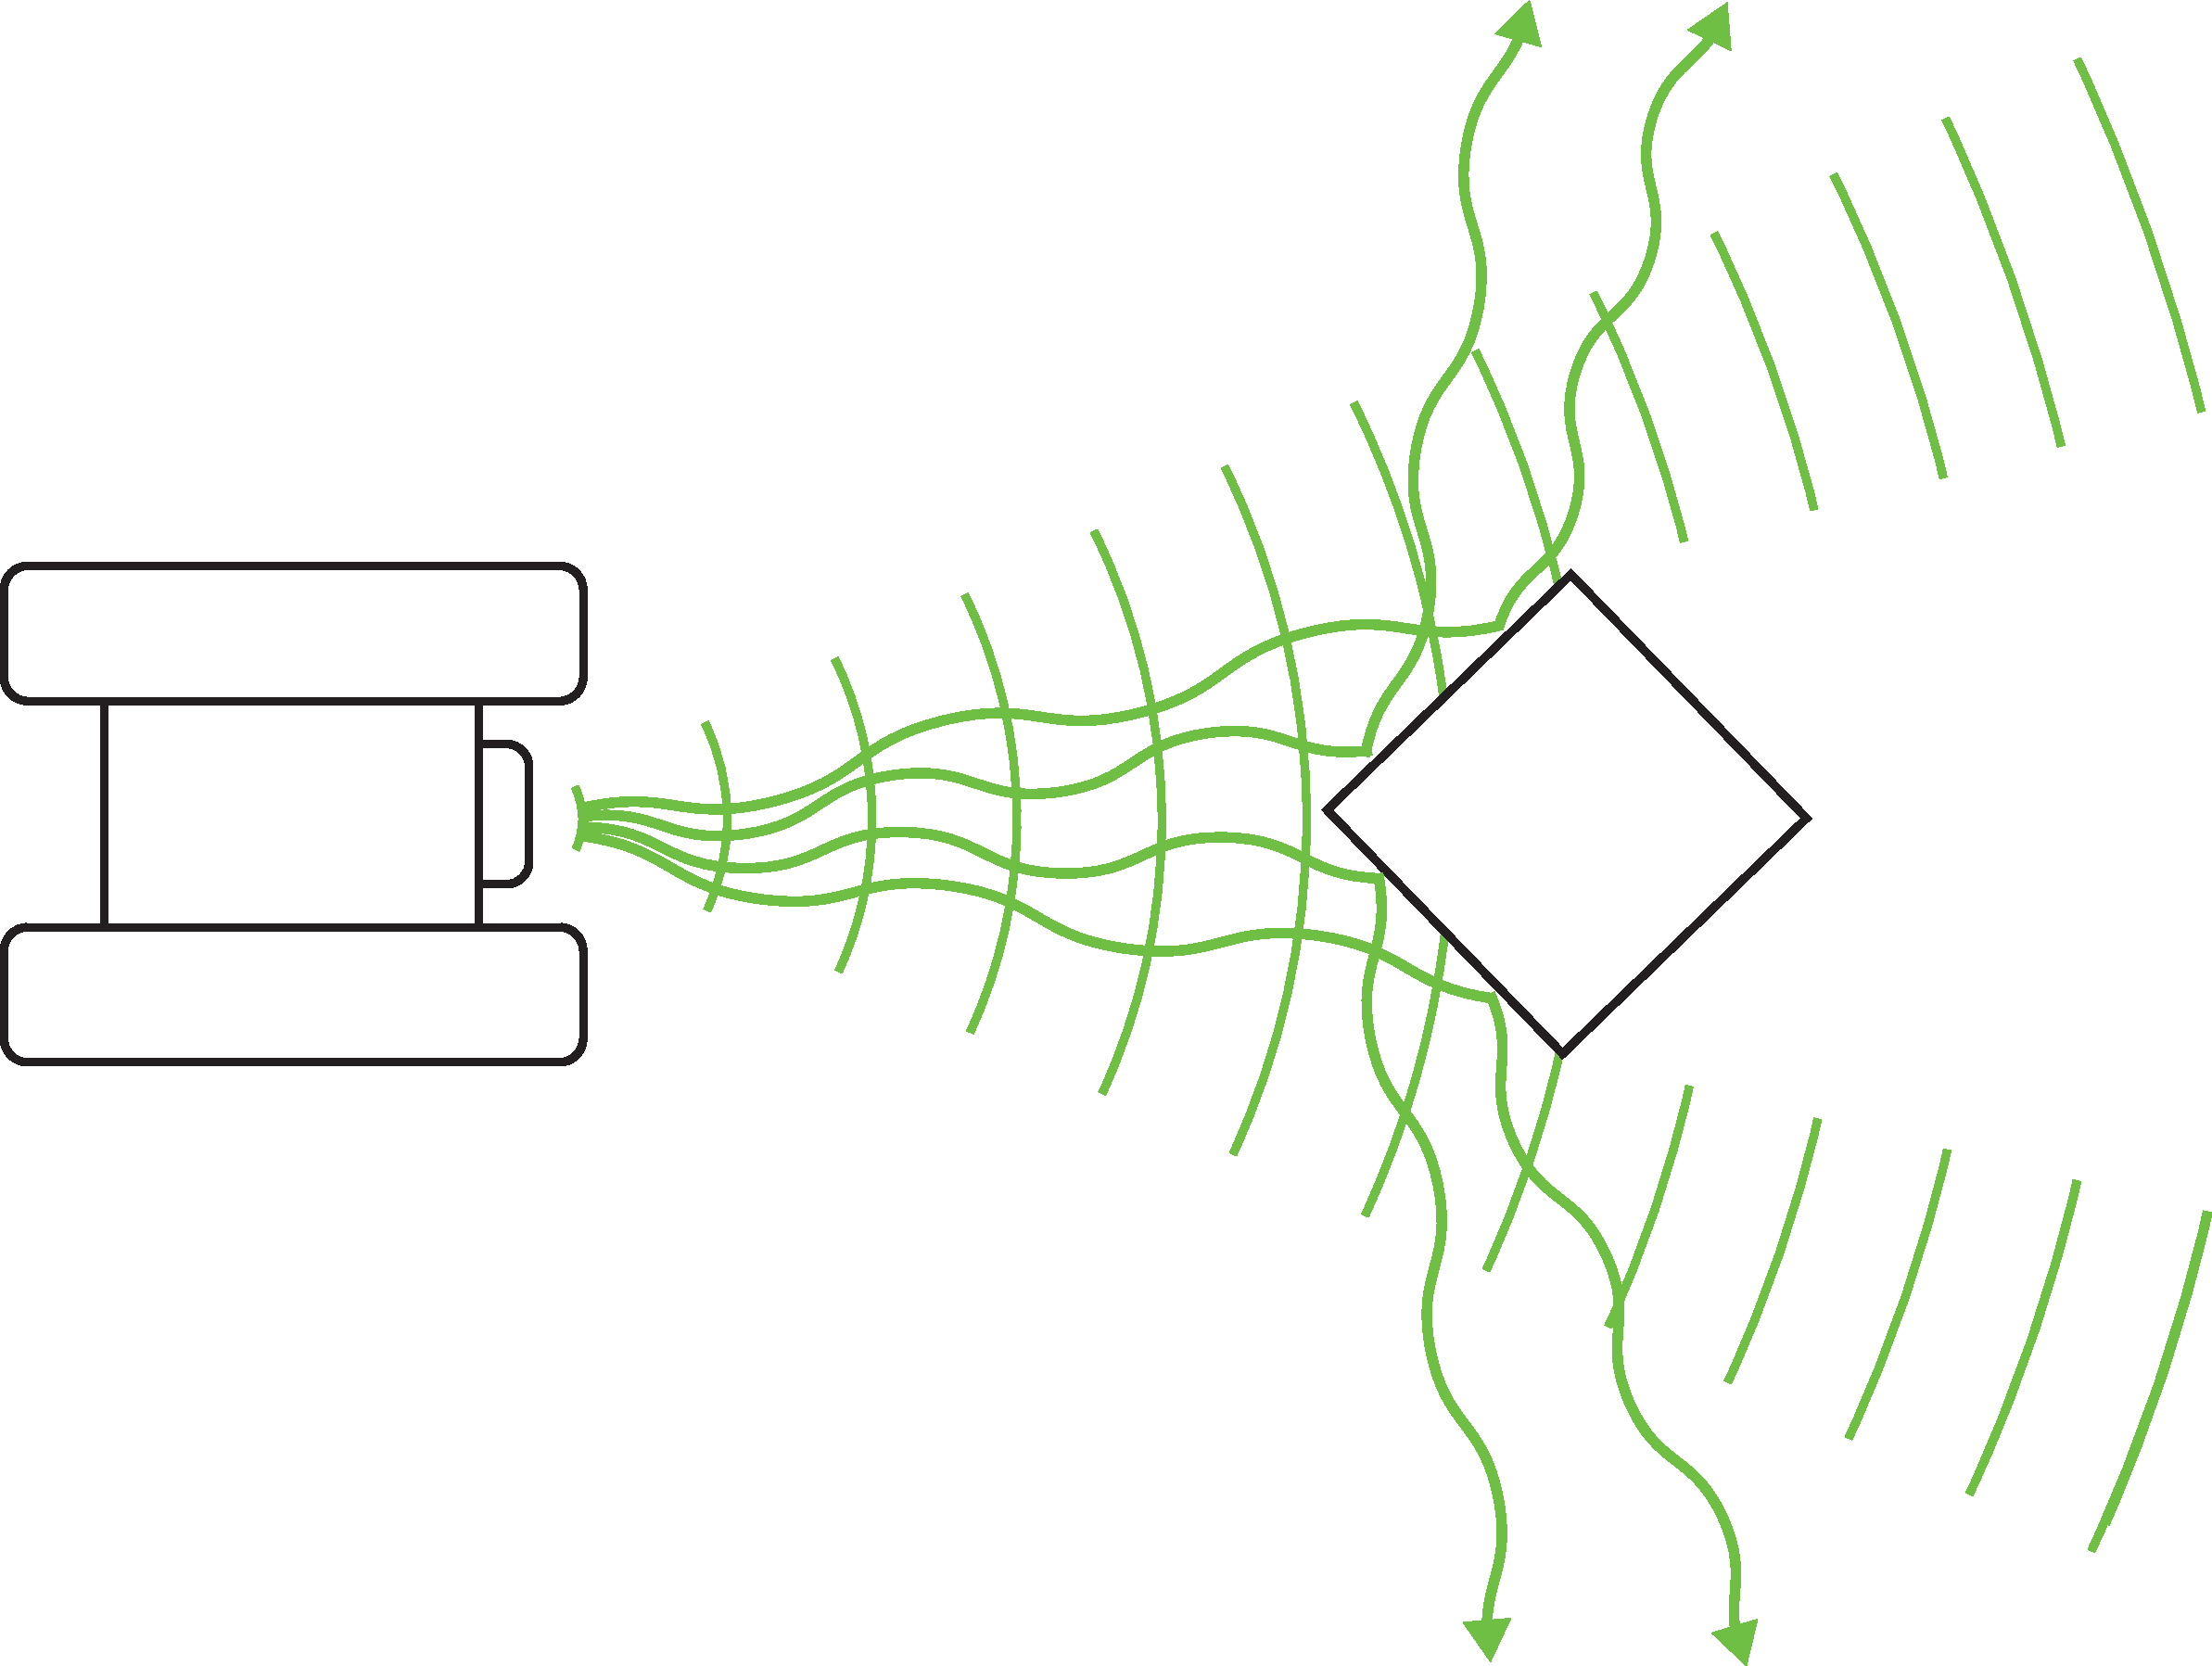
\includegraphics[width=320pt]
     {graphics/SonarWaves.pdf}}
     \caption{\label{fig:angled_object} Sonic waves on an angled object.}
\end{figure}

At short distances, the ultrasonic sensor is proved to be imprecise. This is most highly due to the quality of the sensor and how it is constructed. As seen in \figref{fig:ultrasonic_sensor_test_graph}, the values vary a few cm. The sensor have some problems when it comes to spotting an object at certain angles, for example the angled object illustrated in \figref{fig:angled_object}. The sound waves sent out is reflected away from the sensor. This results in the sensor not being able to correctly calculate the distance and sometimes not being able see the object at all.

\begin{figure}[H]
     \center{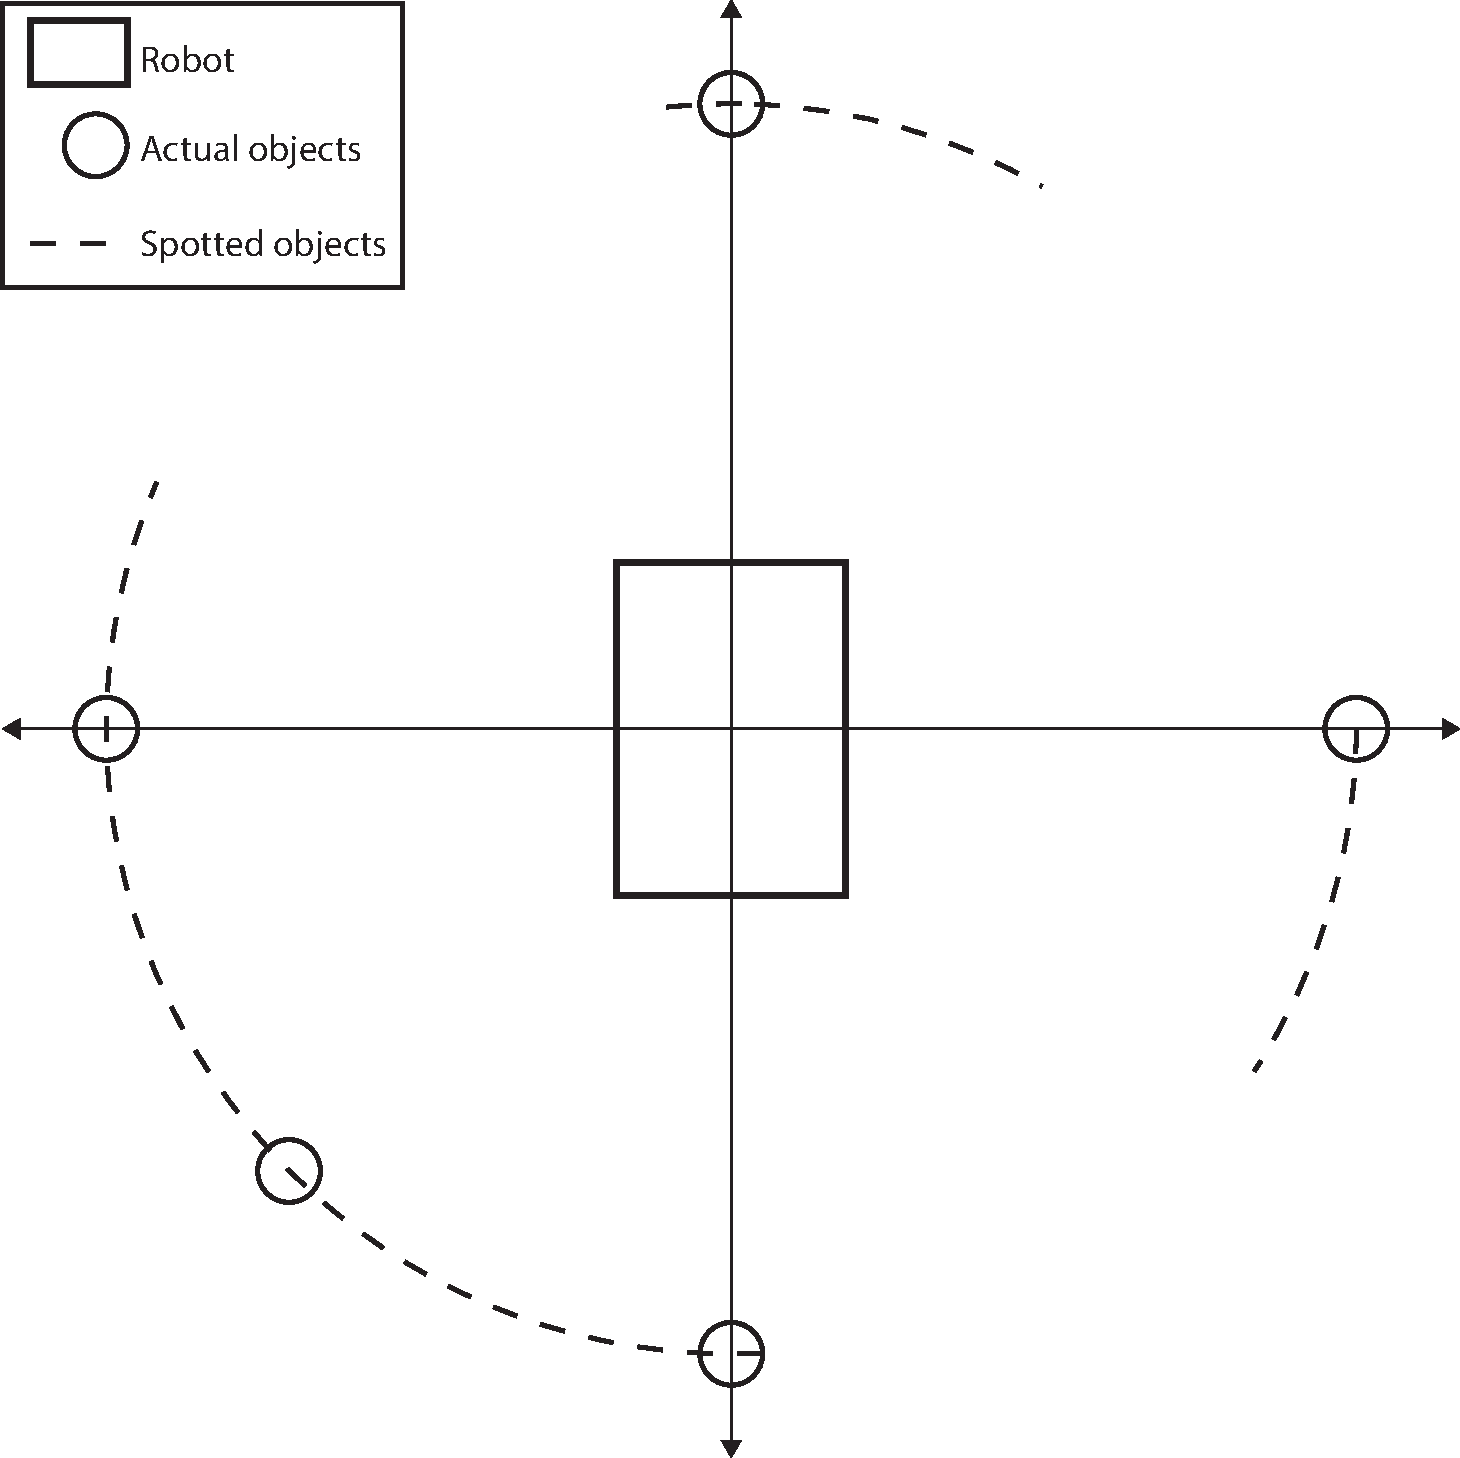
\includegraphics[width=320pt]
     {graphics/SonarTest.pdf}}
     \caption{\label{fig:sonar-test-drawing} 360 degree test with ultrasonic sensor. Graph can be seen in \appref{app:sonar-test-graph}.}
\end{figure}

Last but not least the ultrasonic sensor is having trouble spotting multiple objects if they are standing too close, as seen on the last three objects on \figref{fig:sonar-test-drawing}. It is a matter of the cone being too wide and the first object not being out of sight before the next one is spotted. This results in only one object being added to the object array which means that the \projname{} will get into trouble once it starts collecting.\\
Sometimes the robot is encountering the opposite problem, because sometimes the sound waves does not return despite targeting an object. This break in incoming waves will result in the robot thinking that this is a new object and it will therefore add the same object again.

\subsubsection{Colour sensor} \label{sec:colour_sensor} 
The colour sensor can, by sending out light, measure the reflected light that returns to the sensor. The sensor now contains some raw RGB values, which it can provide the users, or use the integrated colour detecting mechanism to decide which colour it has observed~\citep{lego_education}. 

The test was performed to test the colour sensors ability to detect the black colour which is used as the environment boundary. The sensor should be placed close to the ground, as the only task is to detect the boundary. It should be possible to see a clear difference between the black boundary and the floor. The minimum and maximum values of the black boundary needs to be detected so that \projname{} can distinguish between the floor and the black boundary. Each sensor is tested, where the test provided their respective min and max values after 500 tries. In the end the absolute smallest and largest value is used for each RBG value. This was performed on the boundary and the floor to see the difference between these. A test was also performed, when passing over the black boundary to get the respective values and compare these to the min and max values from the previous test.

\begin{figure}[H]
     \center{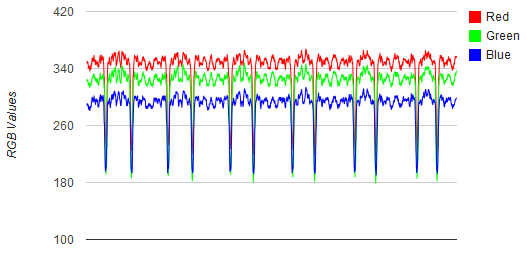
\includegraphics[width=\textwidth]
     {graphics/ColorLeft.png}}
     \caption{\label{fig:colour_sensor_test_left} Graph showing RGB values passing the black boundary 12 times for the left colour sensor.}
\end{figure}

\begin{figure}[H]
     \center{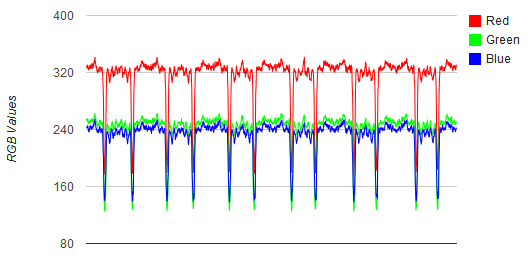
\includegraphics[width=\textwidth]
     {graphics/ColorRight.png}}
     \caption{\label{fig:colour_sensor_test_right} Graph showing RGB values passing the black boundary 12 times for the right colour sensor.}
\end{figure}

As seen on \figref{fig:colour_sensor_test_left} and \figref{fig:colour_sensor_test_right}, the two sensors are quite different when it comes to the values they provide, despite being tested the exact same way. This is important and must be taken into account when using the sensors in the program. Due to uncertainties from the environment such as light, shadows, or dust, even the values in the two figures aren't always accurate. To counter this, it is possible to increase the range between the black minimum and maximum detection values to reduce potential detection problems. This increased range is possible, because the floor RGB values compared with the black values are quite different, allowing the addition of this \emph{extended range}.

\begin{table}[H]
	\centering
	\ra{1.3}
	\rowcolors{3}{Gray}{}
    \begin{tabular}{|l|r|r|r|r|r|r|r|r|}
    \hline
    \rowcolor{DGray}
    \textbf{Sensor} & \multicolumn{4}{c|}{Right} & \multicolumn{4}{c|}{Left} \\ \hline
    \rowcolor{Gray}
    \textbf{Surface} & \multicolumn{2}{c|}{Black boundary} & \multicolumn{2}{c|}{Floor} & \multicolumn{2}{c|}{Black boundary} & \multicolumn{2}{c|}{Floor}   \\ \hline
    \rowcolor{DGray}
    \textbf{Colour range}  & Min~~~~ & Max~~~ & Min~~~ & Max~~~ & Min~~~~ & Max~~~ & Min~~~ & Max~~~ \\ \hline
\multicolumn{1}{|l|}{Red}  & 187     & 260    & 329    & 334    & 209     & 282    & 349    & 354    \\ \hline
\multicolumn{1}{|l|}{Green}& 127     & 192    & 252    & 256    & 173     & 253    & 327    & 332    \\ \hline
\multicolumn{1}{|l|}{Blue} & 147     & 198    & 242    & 248    & 182     & 240    & 292    & 297    \\
    \hline
    \end{tabular}
    \caption{\label{table:colour_sensor_test} Colour sensor results on the black boundary and the floor.}
\end{table}

In~\tblref{table:colour_sensor_test}, the min and max values for each sensor is listed. The values reflect the data on \figref{fig:colour_sensor_test_left} and \figref{fig:colour_sensor_test_right}. These values provide the base line for the RGB value range.


\subsubsection{Compass sensor}
The HiTechnic NXT Compass Sensor is a digital compass that measures the earth's magnetic field and returns a value representing the current heading in degrees. The magnetic heading is returned as an integer from 0 to 359, where 0 is north and 180 is south~\citep{compass}.

The test of the compass sensor is performed the following way: First the sensor is calibrated to work optimally with the \projname{}. The NXT bricks and the motors on the robot have their own magnetic fields which are noise to the compass sensors readings. This makes sensor calibration prior to use a necessity for accurate output values. The compass sensor will furthermore be placed at least 15cm from the motors and 10cm from the NXT bricks~\citep{compass}.

After the initial calibration the robot is placed facing in a direction close to north, which means a heading of around 0 degrees. The robot then performs a 720 degrees spin while the heading is being logged. Turning clockwise the returned value should be a linear increasing value from 0 and up, until 0 degrees is hit again when the robot is facing north. Turning counter-clockwise, the returned value should quickly jump to 359 degrees and linearly decrease while spinning, until north is found again. This will repeat for every 360 degrees the robot does. \fxnote{Sørg for at der står degrees i stedet for cirklen i hele rapporten.}

\begin{figure}[H]
     \center{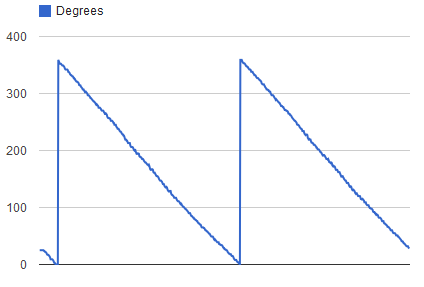
\includegraphics[scale=1]
     {graphics/DegreesGraph.png}}
     \caption{\label{fig:compass_sensor_test_graph} The measured degrees from a 720 degrees counter clockwise turn.}
\end{figure}

\figref{fig:compass_sensor_test_graph} shows the result of a test, where the robot is turning counter-clockwise. The graph illustrates that the compass sensor is outputting the expected values, and thus works as intended. 

\subsubsection{Interactive servo motor} \label{sec:servo_motor}
The LEGO NXT interactive servo motor enables movement. The motors have built-in reduction gear assemblies with internal rotation sensors that measures speed and distance and reports it back to the NXT Brick. This allows for a more precise motor control and the ability to run the motor in steps with one degree of accuracy~\citep{lego_education}.

As the \projname{} has to be able to move around and pick up objects, it would be suitable to drive in a straight line if need be. Therefore the servo motors have been tested to get an idea of a possible difference in performance. The test was set to run for 10 seconds on each motor and measure the degrees of rotation on the specified motor. It was also conducted at different power levels, as the accuracy could vary, depending on the speed. 

\begin{table}[H]
	\centering
	\ra{1.3}
	\rowcolors{1}{Gray}{}
    \begin{tabular}{lccc}
    \hline  
    \rowcolor{DGray}
    \textbf{Power Level}~~~~~~~~~~~~ & Motor L(Degrees) & Motor R(Degrees) & Difference \\ \hline 
    100\%                  & 6,658                  & 6,666                & 0,12\% \\
    90\%                   & 5,823                  & 5,912                & 1,51\% \\
    80\%                   & 5,192                  & 5,262                & 1,33\% \\
    70\%                   & 4,495                  & 4,571                & 1,67\% \\
    60\%                   & 3,859                  & 3,923                & 1,64\% \\
    50\%                   & 3,145                  & 3,211                & 2,07\% \\
    40\%                   & 2,479                  & 2,551                & 2,86\% \\
    \hline 
    \end{tabular}
    \caption{\label{table:servo_motor_test} Servo motor test of rotations.}
\end{table}

As \tblref{table:servo_motor_test} shows, at higher power levels the difference is the smallest, compared to the lower power level, where the difference is increased. This will have an impact on the movement and precision of the \projname{}, therefore this have to be taken into account and adjusted when developing. 

\subsubsection{Object specification} \label{sec:object_specification}
Since the \projname{} is considered a prototype, there are restrictions on the objects it is able to collect. The size of the robot, the strength of the motors and the positions of the objects, all presents some limitations on what objects that can be collected by the \projname{}. The different considerations regarding the objects' attributes are:

\begin{itemize}
\item Size - Can the claw get a hold on the object - and detect it? 
\item Weight - Can the motors lift the object? 
\item Shape - Can it hold the object and not let go?
\item Angle - Can the ultrasonic sensor detect the object from all angles?
\end{itemize}

It is possible to detect objects of 1 cm in width, if the object is placed exactly in the middle of the ultrasonic sensor. If the object is over 12 cm in width, the claw is unable to collect the object. Given the position of the claw compared to that of the ultrasonic sensor, square objects of size 6x6x6 cm, or cylinder objects with a diameter of 6-7 cm are preferred.

Different weight of objects have been tested for the robots strength. The robot's limit is around 150-200 g depending on the object's surface friction. It does not matter if the object weight is close to 0 g, although the robot tend to push around the objects while trying to grab and if the object is too light, there is a risk that it might tip over.

The shape of the object is important; if for instance an object is placed in a way where the ultrasonic sensor's sound waves are not immediately reflected back to the sensor, incorrect values will be provided. Square objects with a sharp corner, are hard to detect and constitute a serious problem to the \projname{}. This is described in \secref{sec:ultrasonic_sensor}. 

If an object is a cylinder, the surface of the object is round, meaning the sound waves are always reflected the same way, no matter how it's angled. This means that it will either always be hard, or always be easy, finding cylindrical objects, since the angle is irrelevant. This has been tested with different kinds of cans and the robot was always able to detect the cans and always returned proper values. It is not enough for the finished product to only work with cylindrical-shaped objects, but for the prototype version of the \projname{}, it is a reasonable restriction.

